\documentclass[a4paper, 12pt]{article}
\usepackage[a4paper,top=1.5cm, bottom=1.5cm, left=1cm, right=1cm]{geometry}
\usepackage{cmap}					
\usepackage{mathtext} 				
\usepackage[T2A]{fontenc}			
\usepackage[utf8]{inputenc}			
\usepackage[english,russian]{babel}
\usepackage{multirow}
\usepackage{graphicx}
\usepackage{wrapfig}
\usepackage{tabularx}
\usepackage{float}
\usepackage{longtable}
\usepackage{hyperref}
\hypersetup{colorlinks=true,urlcolor=blue}
\usepackage[rgb]{xcolor}
\usepackage{amsmath,amsfonts,amssymb,amsthm,mathtools} 
\usepackage{icomma} 
\usepackage{euscript}
\usepackage{mathrsfs}
\usepackage{enumerate}
\usepackage{caption}
\usepackage{enumerate}
\mathtoolsset{showonlyrefs=true}
\usepackage{graphicx}
\usepackage{caption}
\usepackage{subcaption}
\usepackage{amsthm}
\usepackage[europeanresistors, americaninductors]{circuitikz}
\DeclareMathOperator{\sgn}{\mathop{sgn}}
\newcommand*{\hm}[1]{#1\nobreak\discretionary{}
	{\hbox{$\mathsurround=0pt #1$}}{}}

%%% Заголовок

\title{\textbf{Эффект Джоуля-Томсона (2.1.6)}}
\author{Манро Эйден}
\date{}

\begin{document}

\maketitle

\begin{center}
    \section*{Введение}
\end{center}

\noindent \textbf{Цель работы:} 1) Определение изменения температуры углекислого газа при протекании через малопроницаемую перегородку при разных начальных значениях давления и температуры; 2) вычисление по результатам опытов коэффициентов Ван-дер-Ваальса <<a>> и <<b>>.

\bigskip

\noindent \textbf{Оборудование:} трубка с пористой перегородкой; труба Дьюара; термостат; термометры; дифференциальная термопара; микровольтметр; балластный баллон; манометр.

\bigskip

Эффектом Джоуля–Томсона называется изменение температуры газа, медленно протекающего из области высокого в область низкого давления в условиях хорошей тепловой изоляции. В разреженных газах, которые приближаются по своим свойствам к идеальному газу, при таком течении температура газа не меняется. Эффект Джоуля–Томсона демонстрирует отличие исследуемого газа от идеального.
	
	В работе исследуется изменение температуры углекислого газа при медленном его течении по трубке с пористой перегородкой. Трубка 1 хорошо теплоизолирована. Газ из области повышенного давления $P_1$ проходит через множество узких и длинных каналов пористой перегородки 2 в область с атмосферным давлением $P_2$. Перепад давления  $\Delta P = P_1 - P_2$ из-за большого сопротивления каналов может быть заметным даже при малой скорости течения газа в трубке. Величина эффекта Джоуля–Томсона определяется по разности температуры газа до и после перегородки.
	
	Рассмотрим стационарный поток газа между произвольными сечениями I и II трубки (до перегородки и после нее). Пусть, для определенности, через трубку прошел 1 моль углекислого газа; $\mu$ — его молярная масса. Молярные объемы газа, его давления и отнесенные к молю внутренние энергии газа в сечениях I и II обозначим соответственно $V_1$, $P_1$, $U_1$ и $V_2$ , $P_2$ , $U_2$. Для того чтобы ввести в трубку объем $V_1$, над газом нужно совершить работу $A_1$ = $P_1 V_1$. Проходя через сечение II, газ сам совершает работу $A_2$ = $P_2$ $V_2$. Так как через боковые стенки не происходит ни обмена теплом, ни передачи механической энергии, то
	\begin{equation}
		A_1-A_2 = \left(U_2+\frac{\mu v_2^2}{2}\right)-\left(U_1+\frac{\mu v_1^2}{2}\right).
	\end{equation}
	В уравнении (1) учтено изменение как внутренней (первые члены в скобках), так и кинетической (вторые члены в скобках) энергии газа. Подставляя в (1) написанные выражения для $A_1$ и $A_2$ и перегруппировывая члены, найдем
	\begin{equation}
		H_1-H_2 = \left(U + P_1 V_1 \right) - \left(U_2 + P_2 V_2 \right) = \frac{1}{2}\mu\left(v_2^2-v_1^2\right)
	\end{equation}
	
	Сделаем несколько замечаний. Прежде всего отметим, что в процессе Джоуля–Томсона газ испытывает в пористой перегородке существенное трение, приводящее к ее нагреву. Потери энергии на нагрев трубки в начале процесса могут быть очень существенными и сильно искажают ход явления. После того как температура трубки установится и газ станет уносить с собой все выделенное им в пробке тепло, формула (1) становится точной, если, конечно, теплоизоляция трубки достаточно хороша и не происходит утечек тепла наружу через ее стенки.
	
	Второе замечание связано с правой частью (2). Процесс Джоуля–Томсона в чистом виде осуществляется лишь в том случае, если правой частью можно пренебречь, т. е. если макроскопическая скорость газа с обеих сторон трубки достаточно мала. У нас сейчас нет критерия, который позволил бы установить, когда это можно сделать. Поэтому мы отложим на некоторое время обсуждение вопроса о правой части (2), а пока будем считать, что энтальпия газа не меняется.
	
	Рассмотрим выражение:
	\begin{equation}
		\mu_{\text{Д-Т}} = \frac{\Delta T}{\Delta P} \approx \cfrac{\cfrac{2a}{RT}-b}{C_p}
	\end{equation}
	
	Из формулы (3) видно, что эффект Джоуля–Томсона для не очень плотного газа зависит от соотношения величин $a$ и $b$, которые оказывают противоположное влияние на знак эффекта. Если силы взаимодействия между молекулами велики, так что превалирует «поправка на давление», то основную роль играет член, содержащий $a$, и
	\[ \frac{\Delta T}{\Delta P} > 0, \]
	то есть газ при расширении охлаждается ($\Delta t < 0$ так как всегда
	$\Delta P < 0$). В обратном случае (малые a):
	\[ \frac{\Delta T}{\Delta P} < 0, \]
	то есть газ нагревается ($\Delta t < 0$ так как по-прежнему $\Delta P < 0$).
	
	Этот результат нетрудно понять из энергетических соображений. Как мы уже знаем, у идеального газа эффект Джоуля–Томсона отсутствует. Идеальный газ отличается от реального тем, что в нем можно пренебречь потенциальной энергией взаимодействия молекул. Наличие этой энергии приводит к охлаждению или нагреванию реальных газов при расширении. При больших $a$ велика энергия притяжения молекул. Это означает, что потенциальная энергия молекул при их сближении уменьшается, а при удалении — при расширении газа -- возрастает. Возрастание потенциальной энергии молекул происходит за счет их кинетической энергии -- температура газа при расширении падает. Аналогичные рассуждения позволяют понять, почему расширяющийся газ нагревается при больших значениях $b$.
	
	Как следует из формул, при температуре $T_i$ коэффициент $\mu_\text{д-т}$ обращается в нуль. Используя связь между коэффициентами $a$ и $b$ и критической температурой, найдем:
	\begin{equation}
		T_{\text{инв}}=\frac{2a}{bR}, \qquad
		T_{\text{инв}}=\frac{27}{4}T_{\text{кр}}
	\end{equation}
	
	При температуре $T_\text{инв}$ эффект Джоуля–Томсона меняет знак: ниже температуры инверсии эффект положителен ($\mu_\text{д-т} > 0$, газ охлаждается), выше $T_\text{инв}$ эффект отрицателен ($\mu_\text{д-т} < 0$, газ нагревается).	
	
\begin{center}
	\subsection*{Экспериментальная установка}
\end{center}

	\begin{figure}[H]
		\centering{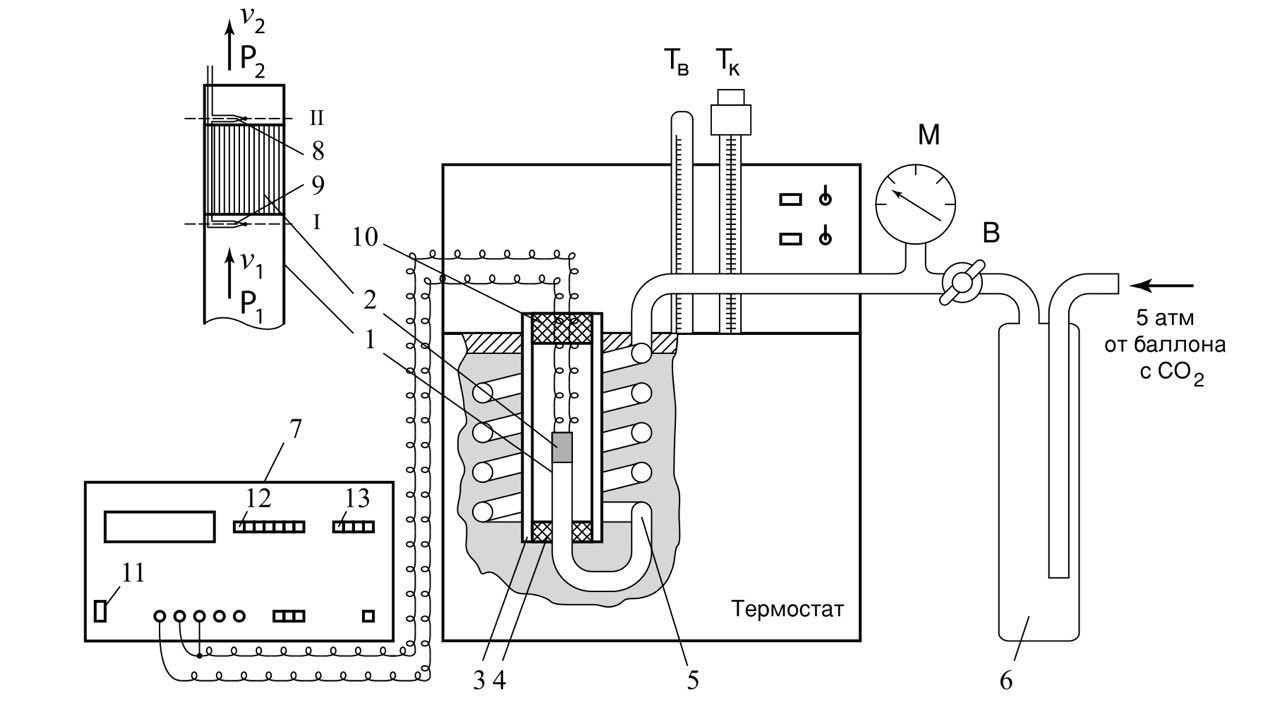
\includegraphics[width=0.75\textwidth]{ust.jpg}}
		\caption[]{\label{ust} Схема установки для изучения эффекта Джоуля–Томсона}
	\end{figure}

	Схема установки для исследования эффекта Джоуля–Томсона в углекислом газе представлена на рисунке \ref{ust}. Основным элементом установки является трубка 1 с пористой перегородкой 2, через которую пропускается исследуемый газ. Трубка имеет длину 80 мм и сделана из нержавеющей стали, обладающей, как известно, малой теплопроводностью. Диаметр трубки $ d = 3 $~мм, толщина стенок 0,2 мм. Пористая перегородка расположена в конце трубки и представляет собой стеклянную пористую пробку со множеством узких и длинных каналов. Пористость и толщина пробки ($ l = 5 $ мм) подобраны так, чтобы обеспечить оптимальный поток газа при перепаде давлений $ \Delta P = 4 $ атм (расход газа составляет около $ 10 $ см$ ^3 $/с); при этом в результате эффекта Джоуля–Томсона создается достаточная разность температур.

	Углекислый газ под повышенным давлением поступает в трубку через змеевик 5 из балластного баллона 6. Медный змеевик омывается водой и нагревает медленно протекающий через него газ до температуры воды в термостате. Температура воды измеряется термометром $ T_\text{в} $, помещенным в термостате. Требуемая температура воды устанавливается и поддерживается во время эксперимента при помощи контактного термометра $ T_\text{к} $.
	
	Давление газа в трубке измеряется манометром М и регулируется вентилем В (при открывании вентиля В, т. е. при повороте ручки против часовой стрелки, давление $ P_1 $ повышается). Манометр М измеряет разность между давлением внутри трубки и наружным (атмосферным) давлением. Так как углекислый газ после пористой перегородки выходит в область с атмосферным давлением $ P_2 $, то этот манометр непосредственно измеряет перепад давления на входе и на выходе трубки $ \Delta P = P_1 - P_2 $.
	
	Разность температур газа до перегородки и после нее измеряется дифференциальной термопарой медь -- константан. Константановая проволока диаметром 0,1 мм соединяет спаи 8 и 9, а медные проволоки (того же диаметра) подсоединены к цифровому вольтметру 7. Отвод тепла через проволоку столь малого сечения пренебрежимо мал. Для уменьшения теплоотвода трубка с пористой перегородкой помещена в трубу Дьюара 3, стенки которой посеребрены, для уменьшения теплоотдачи, связанной с излучением. Для уменьшения теплоотдачи за счет конвекции один конец трубы Дьюара уплотнен кольцом 4, а другой закрыт пробкой 10 из пенопласта. Такая пробка практически не создает перепада давлений между внутренней полостью трубы и атмосферой.
	

\begin{center}
	\subsection*{Погрешности}
\end{center}

\begin{center}
	$\sigma_p = 0,1 \; \text{атм} \; \; \; \; \; \sigma_U = 1 \; \text{мВ} \; \; \; \; \; \sigma_{\varDelta T} = 0,02 \; K$
\end{center}

\newpage

\begin{center}
	\section*{Ход работы}
\end{center}

\begin{table}[H]
	\begin{center}	
		\begin{tabular}{|c|c||c|c||c|c|}
			\hline \hline
			\multicolumn{2}{|c||}{$T = 23 ^\circ C$} & \multicolumn{2}{|c||}{$T = 33 ^\circ C$} &  \multicolumn{2}{|c|}{$T = 43 ^\circ C$} \\ \hline
			$\Delta p$, \text{бар} & $\Delta U$, \text{мкВ} & $\Delta p$, \text{бар} & $\Delta U$, \text{мкВ} & $\Delta p$, \text{бар} & $\Delta U$, \text{мкВ} \\ \hline
			3,9 & 137 & 4,1 & 135 & 4,1 & 135 \\ \hline
			3,7 & 128 & 3,6 & 114 &     &     \\ \hline
			3,2 & 107 & 3,4 & 105 & 3,3 & 68  \\ \hline
			2,8 & 88  & 3,1 & 89  &     &     \\ \hline
			2,3 & 59  & 2,5 & 64  & 2,0 & 38  \\ \hline \hline
		\end{tabular}
	\end{center}
	\label{res}
    \caption {Результаты показаний вольтметра в зависимости от разности давления}
\end{table}

Также для последующей обработки данных необходимо будет учитывать зависимость от температуры чувствительности термопары.

\begin{table}[H]
	\begin{center}
		\begin{tabular}{|c|c|c|c|}
			\hline
			\texxt{Температура}, $^\circ C$ & 20-30 & 30-40 & 40-50 \\ \hline
			\text{мкВ}$/^\circ C$ & 40,7 & 41,6 & 42,5 \\ \hline 
		\end{tabular}
	\end{center}
    \label{sensitivity}
    \caption {Зависимости приведённого напряжения от температуры}
\end{table}

Из наклона графиков найдем соответствующие коэффициенты:

\bigskip

\begin{itemize}
	\item $\displaystyle \mu_{23} = 1,17 \pm 0,05\  K/$\text{бар}, $\displaystyle \sigma_{\mu} = 4\%$;\break
	\item $\displaystyle \mu_{33} = 1,07 \pm 0,03\  K/$\text{бар}, $\displaystyle \sigma_{\mu} = 3\%$;\break
	\item $\displaystyle \mu_{43} = 0,80 \pm 0,04\  K/$\text{бар}, $\displaystyle \sigma_{\mu} = 5\%$;\break
\end{itemize}

Вычислим параметры газа Ван-дер-Ваальса, используя коэффициенты $ \mu_\text{Д--Т} $, полученные для разных пар температур.
Пользуясь формулой (3), получим:

\begin{center}
	$\displaystyle a = \frac{\left(\mu_1 - \mu_2\right)C_PRT_1T_2}{2\left(T_2-T_1\right)}$,\break\break
	$\displaystyle b = \frac{C_P(\mu_2T_2-\mu_1T_1)}{T_1-T_2}. $
\end{center}

После вычислений были получены следующие величины:

\begin{center}
	$\displaystyle a_{23-33}= 1,25 \pm 0,19 \  \frac{\text{Па}\cdot \text{м}^6}{\text{моль}^2}$, $\displaystyle \sigma_{a} = 15 \; \%$; \break

	$\displaystyle a_{33-43}= 3,60 \pm 0,72 \  \frac{\text{Па}\cdot \text{м}^6}{\text{моль}^2}$, $\displaystyle \sigma_{a} = 20 \; \%$; \break

	$\displaystyle b_{23-33}= 6,20 \pm 0,62 \cdot 10^{-5} \ \frac{\text{м}^3}{\text{моль}}$, $\displaystyle \sigma_{b} = 10 \; \%$; \break
	
	$\displaystyle b_{33-43}= 24,0 \pm 3,30 \cdot 10^{-5} \ \frac{\text{м}^3}{\text{моль}}$, $\displaystyle \sigma_{b} = 14 \; \%$. \break
\end{center}
	
Сверим полученные результаты с табличными. Согласно справочнику для углекислого газа

\begin{center}    
	$\displaystyle a = 0,36 \  \frac{\text{Па}\cdot\text{м}^6}{\text{моль}^2}$; \break$\displaystyle b = 4,2\cdot 10^{-5} \ \frac{\text{м}^3}{\text{моль}}.$ 
\end{center}

Полученные данные значительно отличаются от табличных.

Используя формулу (4), по полученным параметрам газа Ван-дер-Ваальса вычислим $ T_\text{инв} $. Также оценим погрешность по следующей формуле:
$\displaystyle \sigma_{T_\text{инв}} = T_\text{инв}\sqrt{\varepsilon^2_a+\varepsilon_b^2}.$

\begin{center}
    $\displaystyle T_{23-33} = 485 K$, $\displaystyle \sigma_{T_{\text{инв}}} = 15\%$; \break
    
    $\displaystyle T_{33-43} = 361 K$, $\displaystyle \sigma_{T_{\text{инв}}} = 15\%$.
\end{center}

Для углекислого газа, согласно справочнику  \[ T_\text{инв} = 2053 \text{ K}.\]

\begin{center}
	\section*{Обсуждение результатов}
\end{center}

\bigskip

Все значения разительно отличаются от табличных. Погрешность вычисления параметров газа Ван-дер-Ваальса составила десятки процентов. Такая боль-
шая ошибка говорит нам о неприменимости уравнения Ван-дер-Ваальса в усло-
вия лабораторной работы. Действительно, это уравнение используется лишь для каче-
ственного описания процессов, происходящих с реальными газами. Количественный под-
ход к этому уравнению неприменим. Большую погрешность составил барометр.

\bigskip

\begin{center}
	\section*{Вывод}
\end{center}

Наша модель плохо описывает поведение системы, поскольку финальные коэффициенты не сошлись с табличными. Не смотря на это, они отличались от них меньше, чем в 20 раз, что не так плохо. Мы измерили изменение температуры углекислого газа при протекании через перегородку при различных давлениях и температурах и вычеслили значения коэффициентов Ван-дер-Ваальса и температуры инверсии, хоть и не точно.

\end{document}